% ----------------------------------------------------------------------------------------------------------
% Praeambel
% ----------------------------------------------------------------------------------------------------------
\documentclass[fontsize=12pt,%
paper=a4,%
%DIV=calc,%
%BCOR=10mm,%
twoside=false,%
headings=openany,%
parskip=half,%
pagesize=auto,%
numbers=noenddot,%
headsepline=true,%
toc=listof,%
toc=bibliography%
]{scrreprt}

% PDF-Kompression
\pdfminorversion=5
\pdfobjcompresslevel=1

%\usepackage{marginnote}

\usepackage{geometry}
\geometry{a4paper,left=40mm,right=25mm, top=25mm, bottom=25mm, includeheadfoot}

\usepackage{makeidx}
\makeindex
\usepackage{tikz}
\usepackage{epstopdf} 
%\usepackage[language=German]{chemmacros}

% Schriften
%\RequirePackage{mathptmx}%
%\RequirePackage[scaled=0.95]{helvet}%
%\renewcommand\familydefault{\sfdefault}%
\usepackage{mathpazo,tgpagella}
%\usepackage{libertine}
%\usepackage{fourier}
\usepackage{lmodern}

\usepackage{blindtext}
\usepackage{pdfpages}
% Allgemeines
\usepackage{amsmath,amssymb} % Mathesachen
\usepackage[T1]{fontenc} % Ligaturen, richtige Umlaute im PDF
% UTF8-Kodierung für Umlaute usw
\usepackage[utf8]{inputenc}

\usepackage[decimalsymbol=comma]{siunitx}
\usepackage{scrlayer-scrpage} 
\pagestyle{scrheadings}

\usepackage{setspace}
\onehalfspacing 

% Schriften-Größen
\setkomafont{chapter}{\huge\rmfamily}
\setkomafont{section}{\Large\rmfamily}
\setkomafont{subsection}{\large\rmfamily}
\setkomafont{subsubsection}{\large\rmfamily}
\setkomafont{chapterentry}{\large\rmfamily} % Überschrift der Ebene in Inhaltsverzeichnis
\setkomafont{descriptionlabel}{\bfseries\rmfamily} % für description Umgebungen
\setkomafont{captionlabel}{\small\bfseries}
\setkomafont{caption}{\small}

% Sprache: Deutsch
\usepackage[autostyle,babel,german=guillemets,style=german]{csquotes}
\usepackage[USenglish,ngerman]{babel} 
\selectlanguage{ngerman}
% PDF
\usepackage[ngerman,%
pdfauthor={Benjamin Ternes},%
pdftitle={Metadaten für die PDF},%
colorlinks=true,linkcolor=black,citecolor=black,filecolor=black,urlcolor=black%
]{hyperref}

% BibLaTeX
\usepackage[backend=biber,%
 style=alphabetic,%
 %bibstyle=numeric,%
 %citestyle=numeric,%
 % autocite=inline,%
 sorting=anyt,%
 sortcites=true,%
 hyperref=auto,%
 maxnames=2,%
 minnames=1,%
]{biblatex}

\bibliography{_bibliography/biblio.bib}

\setlength{\bibitemsep}{1em}
\DefineBibliographyStrings{ngerman}{andothers = {u.\,a.},}
%\defbibheading{head}{\addchap{Literaturverzeichnis}}

\usepackage[final]{microtype} % mikrotypographische Optimierungen
\usepackage{url}
\usepackage{pdflscape} % einzelne Seiten drehen können
\usepackage{hyperref}
%  Bibliographie
%\usepackage{bibgerm} % Umlaute in BibTeX

% Tabellen
\usepackage{multirow} % Tabellen-Zellen über mehrere Zeilen1
\usepackage{multicol} % mehre Spalten auf eine Seite
\usepackage{tabularx} % Für Tabellen mit vorgegeben Größen
\usepackage{array}
\usepackage{float}
\usepackage{booktabs}
\usepackage{longtable} % Tabellen über mehrere Seiten

% Bilder
\usepackage{graphicx}
\usepackage{color}

\graphicspath{{_img/}}
\DeclareGraphicsExtensions{.pdf,.png,.jpg}

\usepackage{subfigure}
\newcommand{\subfigureautorefname}{\figurename}

\usepackage[all]{hypcap}

\newcommand{\longpage}{\enlargethispage{\baselineskip}}
\newcommand{\verylongpage}{\enlargethispage{2\baselineskip}}
\newcommand{\shortpage}{\enlargethispage{-\baselineskip}}
\newcommand{\veryshortpage}{\enlargethispage{-2\baselineskip}}

% Bildunterschrift
\setcapindent{0em}
\setcapwidth[c]{0.9\textwidth}
\setlength{\abovecaptionskip}{0.2cm}

% Quellcode
\usepackage{listings}
\definecolor{mygreen}{RGB}{28,172,0} 		% color values Red, Green, Blue
\definecolor{mylilas}{RGB}{170,55,241}
\lstset{language=Matlab,%
	basicstyle=\footnotesize\ttfamily,
	breaklines=true,%
	morekeywords={matlab2tikz},
	keywordstyle=\color{blue},%
	morekeywords=[2]{1}, keywordstyle=[2]{\color{black}},
	identifierstyle=\color{black},%
	stringstyle=\color{mylilas},
	commentstyle=\color{mygreen},%
	showstringspaces=false,%without this there will be a symbol in the places where there is a space
	numbers=left,%
	numberstyle={\tiny \color{black}},% size of the numbers
	numbersep=9pt, % this defines how far the numbers are from the text
	emph=[1]{for,end,break},emphstyle=[1]\color{red}, %some words to emphasise
	%emph=[2]{word1,word2}, emphstyle=[2]{style},    
}

% linksbündige Fußboten
\deffootnote{1.5em}{1em}{\makebox[1.5em][l]{\thefootnotemark}}


%\typearea{14} % typearea berechnet einen sinnvollen Satzspiegel (das heißt die Seitenränder) siehe auch http://www.ctan.org/pkg/typearea. Diese Berechnung befindet sich am Schluss, damit die Einstellungen oben berücksichtigt werden
% für autoref von Gleichungen in itemize-Umgebungen
\makeatletter
\newcommand{\saved@equation}{}
\let\saved@equation\equation
\def\equation{\@hyper@itemfalse\saved@equation}
\makeatother 

\usepackage[framemethod=TikZ]{mdframed}
\usepackage{xcolor}

\definecolor{light-gray}{gray}{0.85}
%\definecolor{lightblue}{blue}{0.35}

\newmdenv[%
    backgroundcolor=light-gray,
    linecolor=light-gray,
    outerlinewidth=2pt,
    roundcorner=2mm,
    skipabove=\baselineskip,
    skipbelow=\baselineskip,
]{shaded}

\usepackage{acronym}

\newcommand{\myquote}[3]{\begion{quote}\enquote{#1~\autocite[S.~#2]{#3}}}

\usepackage{xspace} 
\newcommand{\AdV}{Anm.\ d.\ Verf.\@\xspace}
\newcommand{\bzw}{beziehungsweise\@\xspace}
\newcommand{\etc}{etc.\@\xspace}
\newcommand{\bspw}{beispielsweise\@\xspace}
\newcommand{\bzgl}{bzgl.\@\xspace}
\newcommand{\ea}{et\,al.\@\xspace}
\newcommand{\etal}{et\,al.\@\xspace} 
\newcommand{\latex}{\LaTeX\@\xspace}
\newcommand{\insb}{insbesondere\@\xspace}
\newcommand{\dH}{das heißt\@\xspace}
\newcommand{\ggf}{gegebenenfalls\@\xspace}
\newcommand{\ggfs}{gegebenenfalls\@\xspace}
\newcommand{\idR}{in der Regel\@\xspace}
\newcommand{\ivm}{i.\,V.\,m.\@\xspace}
\newcommand{\ieS}{i.\,e.\,S.\@\xspace}
\newcommand{\is}{i.\,S.\@\xspace}
\newcommand{\iwS}{i.\,w.\,S.\@\xspace}
\newcommand{\oae}{o.\,{\"a}.\@\xspace}
\newcommand{\og}{o.\,g.\@\xspace}
\newcommand{\ua}{u.\,a.\@\xspace}
\newcommand{\uae}{u.\,{\"a}.\@\xspace}
\newcommand{\usw}{usw.\@\xspace}
\newcommand{\uU}{u.\,U.\@\xspace}
\newcommand{\uvm}{u.\,v.\,m.\@\xspace}
\newcommand{\va}{v.\,a.\@\xspace}
\newcommand{\zB}{\mbox{zum Beispiel}\@\xspace}
\newcommand{\zt}{z.\,T.\@\xspace}
\newcommand{\vglzb}{vgl.\,z.\,B.\@\xspace}
\newcommand{\vgl}{vergleiche\@\xspace}
\newcommand{\sog}{so genannt\@\xspace}
\newcommand{\so}{siehe oben\@\xspace}
\newcommand{\msc}{M.\,Sc.\@\xspace}
\newcommand{\bsc}{B.\,Sc.\@\xspace}

\newcommand{\x}[1]{\mathrm{#1}}
\newcommand{\y}[1]{\ch{#1}}

\usepackage{blindtext}

\usepackage{chemformula,chemmacros}
\renewtagform{reaction}[R ]{[}{]}

% Endredaktion

%\clubpenalty = 9000
%\widowpenalty = 9000
%\displaywidowpenalty = 9000

\newcommand{\fat}[1]{{\textbf{#1}}}

\newcommand{\todo}[1]{
	{\colorbox{light-gray}{ TODO: #1 }}
}

\newcommand{\todotext}[1]{
	{\color{red} TODO: #1} \normalfont
}

\newcommand{\info}[1]{
	{\colorbox{blue}{ (INFO: #1)}}
}
 
\usepackage{tikz}
\definecolor{c100f0d}{RGB}{16,15,13}

\begin{document}
\pagestyle{empty}
\cleardoublepage
% ----------------------------------------------------------------------------------------------------------
% Titelseite
% ----------------------------------------------------------------------------------------------------------
\clearscrheadings\clearscrplain

\section*{Sperrvermerk}

\textcolor{red}{
Die vorliegende Arbeit \enquote{Titel der Arbeit} beinhaltet auch vertrauliche Informationen der Firma XX.
Die Veröffentlichung und/oder Weitergabe des Inhalts der Arbeit im Gesamten oder in Teilen sowie das Anfertigen von Kopien oder Abschriften~--~auch in digitaler Form~--~sind grundsätzlich untersagt.
Ausnahmen bedürfen der vorherigen schriftlichen Zustimmung der Firma XX.}

\vspace{10cm}

\begin{displaymath}
\begin{array}{ll}
Unterschrift:~~~~~~~~~~~~~~~~~~~~~~~~~~~~~~~~~~~~~~~~~~
& Ort, Datum:~~~~~~~~~~~~~~~~~~~~~~~~~~~~~~~~~~~~~~~~~~
\end{array}
\end{displaymath}





\cleardoublepage
\clearscrheadings\clearscrplain

\begin{titlepage}
	
\begin{center}
	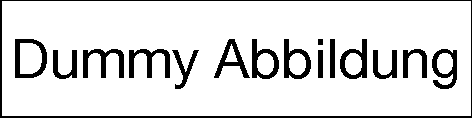
\includegraphics[width=0.5\textwidth]{_images/logo}
\end{center}

\begin{center}
	%\vspace*{4cm}
	
	\Huge
	\textbf{Masterarbeit}\\
	\vspace*{0.5cm}
	\large
	zur Erlangung des akademischen Grades\\
	Master of Science (M.Sc.)\\
	\vspace*{1cm}
	\huge
	\textbf{Vorlage für Abschlussarbeiten in \LaTeX}\\
	\vspace*{2cm}
	\vfill
	\normalsize
	\newcolumntype{x}[1]{>{\raggedleft\arraybackslash\hspace{0pt}}p{#1}}
	
	\begin{tabular}{x{6cm}p{7.5cm}}
		\rule{0mm}{5ex}\textbf{Autor:} & Benjamin Ternes\newline benjamin.ternes@fernuni-hagen.de\newline Matrikelnummer: XXXXX\\
		\rule{0mm}{5ex}\textbf{Erstgutachter:} & Prof.\ Dr.-Ing.\ XXX \\
		\rule{0mm}{2ex}\textbf{Zweitgutachter:} & Prof.\ Dr.-Ing.\ XXX \\ 
		\rule{0mm}{5ex}\textbf{Abgabedatum:} & Tag.~Monat~Jahr \\ 
	\end{tabular} 
\end{center}
\end{titlepage}

\cleardoublepage

\dictum{Man merkt nie, was schon getan wurde, man sieht immer nur, was noch zu tun bleibt. (Marie~Curie, *7.\ November 1867~--~$\dagger$ 4.\ Juli 1934)\\ \vspace{1cm} Eine neue wissenschaftliche Erkenntnis lässt sich gewöhnlich nicht so darstellen, dass ihre Gegner überzeugt sind. Diese sterben vielmehr aus, und eine nachwachsende Generation ist von Anfang an mit der Wahrheit vertraut. (Max~Planck, *23.\ April 1858~--~$\dagger$ 4.\ Oktober 1947)}

\cleardoublepage

\clearscrheadings\clearscrplain
\chapter*{Danksagung}

\blindtext[2]

\cleardoublepage

\pagestyle{scrheadings}
\ohead[]{\pagemark}
\ihead[]{\headmark}
\ifoot[]{}
\automark[chapter]{chapter}
\automark*[section]{section}
%\renewcommand*{\chapterpagestyle}{scrheadings}

%\cleardoublepage
\pagenumbering{roman}
% ----------------------------------------------------------------------------------------------------------
% Verzeichnisse
% ----------------------------------------------------------------------------------------------------------
%\addcontentsline{toc}{chapter}{Inhaltsverzeichnis}
\tableofcontents

\cleardoublepage
% ----------------------------------------------------------------------------------------------------------
% Einleitung
% ----------------------------------------------------------------------------------------------------------

\addchap{Abkürzungsverzeichnis}
\begin{acronym}[PMSM]	% längste Abkürzung
	\acro{PMSM}{Permanentmagneterregte Synchronmaschine}
	\acro{GSM}{Gleichstrommaschine}
	\acro{ASM}{Asynchronmaschine}
\end{acronym}

\cleardoublepage

\addchap{Symbolverzeichnis}
\begin{tabularx}{\textwidth}{p{0.2\textwidth}p{0.5\textwidth}p{0.3\textwidth}}
	\toprule
	Symbol & Bedeutung & Einheit \\
	\midrule
	$E$			& Elektrische Feldstärke				& \si{\volt\per\meter} \\
	$D$			& Elektrische Flussdichte				& \si{\ampere\second\per\square\meter} \\
	$H$			& magnetische Feldstärke				& \si{\ampere\per\meter} \\
	$B$			& magnetische Flussdichte				& \si{\tesla} \\
	\bottomrule
\end{tabularx}	

\cleardoublepage

\thispagestyle{empty}
\pagenumbering{arabic}
\section*{Kurzfassung}

\blindtext[1]

\section*{Abstract}

\blindtext[1]
\pagestyle{scrheadings}
% ----------------------------------------------------------------------------------------------------------
% Kapitel
% ----------------------------------------------------------------------------------------------------------

\cleardoublepage

% -*- coding: utf-8 -*-
% !TEX encoding = UTF-8 Unicode
% !TEX root =  main.tex

\chapter{Beispiel Kapitel}
\label{chap:beispiel-kapitel}

\section{Abbildungen}\label{sec:abbildungen}

Eine Abbildung lässt sich einfach über:

\lstset{language=TeX}
\begin{lstlisting}
\begin{figure}[htb]
\includegraphics{..pfad/foc-ac-dc.pdf}
\caption{Beschriftung der Abbildung}
\label{fig:foc-ac-dc}
\end{figure}
\end{lstlisting}

einfügen.
Die breite der Abbildung kann einerseits skaliert oder direkt im Maßstab von \SI{14.5}{\centi\meter} erstellt werden.
Wenn die Abbildung maßstabsgetreu erstellt wird, muss \verb|\centering| und der optionale Befehl \verb|[width=\textwidth]| nicht zwingend übernommen werden.

\begin{figure}[htb]
	\centering
	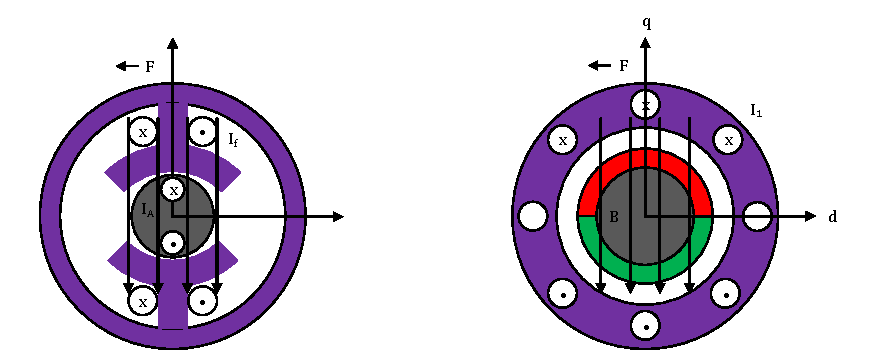
\includegraphics[width=\textwidth]{_images/chapter1/foc-dc-ac.pdf}
	\caption{Beschriftung der Abbildung}
	\label{fig:foc-dc-ac}
\end{figure}

Für Zitationen wird \verb|BibLaTeX| verwendet. Als Backend wird \verb|biber| vom Kompiler verlangt.
Biber ist Open Source und kann im CTAN Repository heruntergeladen werden: \url{https://www.ctan.org/pkg/biber}.

\begin{quote}
\enquote{Bei jeder permanentmagneterregten Synchronmaschine ändern sich die Induktivitäten in abhängigkeit von der Last. In erster Linie sind dafür die Sättigungseffekte, aber auch die Kreuzkopplung verantwortlich.} \autocite[S.~2]{ternes2015}
\end{quote}

Im Text zitierte Werke werden über die Syntax \verb|\textcite[S.~2]{ternes2015}| korrekt zitiert. Beispielsweise: Wie in \textcite[S.~2]{ternes2015} erläutert, sind die Induktivitäten abhängig von der Last \ldots

Der aktuelle Stil des Literaturverzeichnisses und der Zitationen ist \verb|alphabetic|, kann aber auch in Absprache geändert werden, dazu empfiehlt es sich, die \verb|BibLaTeX|-Dokumentation zu konsultieren.

\section{Literaturverwaltungsprogramme}

Die Verwaltung des Lizeraturverzeichnisses stellt bei Abschlussarbeiten eine große Herausforderung dar. Um vermeidbaren Fehlern vorzubeugen empfiehlt sich die Nutzung einer sog.\ Literaturverwaltungssoftware. In den meisten Fällen ist ein direkte Export als \verb|biblatex|-Datei integriert, was das einbinden in die Abschlussarbeit deutlich erleichtert.  

\begin{table}[htb]
	\caption{Einführender Überlick über Literaturverwaltungsprogramme}
	\label{tab:literaturverwaltung}
	\begin{tabularx}{1.0\textwidth}{l l l X}
		\toprule
			Programm & OS & Website & Extras\\
		\midrule
			Zotero & Windows, OS X & \href{https://www.zotero.org}{zotero.org} & FireFox Plugin, ISBN Suchfunktion\\
			Mendeley & Windows, OS X & \href{https://www.mendeley.com/}{mendeley.com} & watchfolder\\
			JabRef	& Windows, OS X & \href{http://jabref.sourceforge.net/}{jabref} & natives bibtex Format \\
		\bottomrule
	\end{tabularx}
\end{table}

\section{Tabellen}\label{sec:tables}

Die folgende Tabelle (s.~Tab.~\ref{tab:tabelle-test}) ist ein Beispiel.

\begin{table}[htb]
		\caption{Tabellenüberschrift}
		\label{tab:tabelle-test}
		\centering
	\begin{tabularx}{0.4\textwidth}{l c c}
			\toprule
			Messsung	&	Spannung		&	Strom	\\
			&	\si{\volt}	&	\si{\ampere} \\
			\midrule
			1			&	12.2			&	1.2	\\
			2			&	13.1			&	1.21 \\
			\bottomrule
	\end{tabularx}
\end{table}



\section{Abschließende Hinweise zum anfertigen von wissenschaftlichen Qualifikationsarbeiten}\label{sec:hinweise-wiss-arbeiten}

 Um die Leserlichkeit eines Textes zu verbessern sollten einige typografische Regeln beachtet werden. Eine einführende Lektüre hierfür ist: \fullcite{bier_typokurz_2009}. Bevor Sie sich mit dieser Vorlage auseinadersetzen, sollten Sie dieses Werk gelesen haben.
 
 Für die Einführung in das wissenschaftliche arbeiten mit \LaTeX\ empfehle ich folgendes Buch: \fullcite{schlosser_wissenschaftliche_2014}. Dieses Buch dient lediglich als Einführung und dient dem besseren Verständnis und Umgang mit \LaTeX.
 
 Als \enquote{Standardwerk} für das wissenschaftliche Arbeiten empfehle ich: \fullcite{theisen_wissenschaftliches_2013}.

Das folgende Buch: \fullcite{kornmeier_wissenschaftlich_2013}, ist eine Art \enquote{Kochbuch} für das wissenschaftliche Arbeiten und versucht dieses auch zu vermitteln. Für eine differenzierte Betrachtung empfehle ich die Auseinandersetzung mit anderer Fachliteratur in diesem Bereich.

%%% Local Variables: 
%%% mode: latex
%%% TeX-master: "main.tex"
%%% TeX-open-quote: "\\enquote{"
%%% TeX-close-quote: "}"
%%% LaTeX-csquotes-open-quote: "\\enquote{"
%%% LaTeX-csquotes-close-quote: "}"
%%% End: 

%\input{_content/Kapitel-1}
%\input{_content/Kapitel-2}
%\input{_content/Kapitel-3}
%\input{_content/Kapitel-4}

% ----------------------------------------------------------------------------------------------------------
% Verzeichnisse
% ----------------------------------------------------------------------------------------------------------
\cleardoublepage
\pagenumbering{Roman}
\cleardoublepage
\listoffigures
\cleardoublepage
\listoftables
\cleardoublepage
%\listofreactions
%\renewcommand{\indexname}{Stichwortverzeichnis}
%\addcontentsline{toc}{chapter}{Stichwortverzeichnis}
%\printindex
% ----------------------------------------------------------------------------------------------------------
% Literatur
% ----------------------------------------------------------------------------------------------------------
\cleardoublepage
\nocite{*}
\printbibliography
% ----------------------------------------------------------------------------------------------------------
% Anhang
% ----------------------------------------------------------------------------------------------------------
\cleardoublepage

\begin{appendix}
\chapter{Anhang}


 
\end{appendix}

\cleardoublepage
\section*{Eidesstattliche Erklärung}
\thispagestyle{empty}

\begin{verbatim}

\end{verbatim}

\begin{LARGE}
	
	Eidesstattliche Erklärung zur Abschlussarbeit:
	
	\enquote{Titel der Arbeit}
	
\end{LARGE}

\begin{verbatim}


\end{verbatim}
Ich versichere, die von mir vorgelegte Arbeit selbstständig verfasst zu haben. Alle Stellen, die wörtlich oder sinngemäß aus veröffentlichten oder nicht veröffentlichten Arbeiten anderer entnommen sind, habe ich als entnommen kenntlich gemacht. Sämtliche Quellen und Hilfsmittel, die ich für die Arbeit benutzt habe, sind angegeben. Die Arbeit hat mit gleichem Inhalt bzw. in wesentlichen Teilen noch keiner anderen Prüfungsbehörde vorgelegen.



\begin{displaymath}
% use packages: array
\begin{array}{ll}
Unterschrift:~~~~~~~~~~~~~~~~~~~~~~~~~~~~~~~~~~~~~~~~~~
& Ort, Datum:~~~~~~~~~~~~~~~~~~~~~~~~~~~~~~~~~~~~~~~~~~
\end{array}
\end{displaymath}


\end{document}